% Bản tiếng Việt của main.tex, chỉ để đọc (không nộp). Biên dịch: xelatex main_vi; bibtex main_vi; xelatex main_vi x2.
% Luật viết: skill upar-paper-rules. Thuật ngữ giữ tiếng Anh theo PLAN.md (encoder, query head, attention head, ...).
\documentclass[10pt,twocolumn,letterpaper]{article}

\usepackage[review,algorithms]{wacv}
\usepackage{fontspec}
\setmainfont{Liberation Serif}
\setsansfont{Liberation Sans}

%
% --- inline annotations
%
\newcommand{\red}[1]{{\color{red}#1}}
\newcommand{\todo}[1]{{\color{red}#1}}
\newcommand{\TODO}[1]{\textbf{\color{red}[TODO: #1]}}
% --- disable by uncommenting  
% \renewcommand{\TODO}[1]{}
% \renewcommand{\todo}[1]{#1}


\usepackage{booktabs}
\usepackage{amsmath}
\usepackage{graphicx}
\graphicspath{{figs/}}

\definecolor{wacvblue}{rgb}{0.21,0.49,0.74}
\usepackage[pagebackref,breaklinks,colorlinks,allcolors=wacvblue]{hyperref}
\usepackage[capitalize]{cleveref}
% wacv.sty sets the cleveref names at the end of the preamble, so the Vietnamese names go in \AtBeginDocument
\AtBeginDocument{%
\crefname{section}{Mục}{Mục}\Crefname{section}{Mục}{Mục}%
\crefname{subsection}{Mục}{Mục}\Crefname{subsection}{Mục}{Mục}%
\crefname{figure}{Hình}{Hình}\Crefname{figure}{Hình}{Hình}%
\crefname{table}{Bảng}{Bảng}\Crefname{table}{Bảng}{Bảng}%
\crefname{equation}{Pt.}{Pt.}\Crefname{equation}{Pt.}{Pt.}%
\renewcommand{\crefpairconjunction}{ và }%
\renewcommand{\crefmiddleconjunction}{, }%
\renewcommand{\creflastconjunction}{ và }%
}
\renewcommand{\figurename}{Hình}
\renewcommand{\tablename}{Bảng}
\renewcommand{\refname}{Tài liệu tham khảo}
\def\elvbf{\fontsize{11}{13}\selectfont\bfseries}\def\tenbf{\fontsize{10}{12}\selectfont\bfseries}
\def\abstract{\centerline{\large\bf Tóm tắt}\vspace*{12pt}\noindent\it\ignorespaces}

\def\wacvPaperID{*****}
\def\confName{WACV}
\def\confYear{2027}

\title{UniQuery: Hợp nhất các vision model bằng một Joint Query Head\\cho nhận dạng thuộc tính người đi bộ xuyên domain}
\author{Bản tiếng Việt để đọc nội bộ (không nộp)}

\begin{document}
\maketitle

%=====================================================================
\begin{abstract}
Bài báo này trình bày giải pháp của nhóm cho Track~1, nhận dạng thuộc tính người đi bộ (Pedestrian Attribute Recognition, PAR), của UPAR Challenge 2027 tại workshop Real-World Surveillance của WACV 2027. PAR cho ra mô tả ngữ nghĩa của từng người, phục vụ truy vấn người theo thuộc tính và hỗ trợ tái nhận dạng người. Tuy vậy, nhận dạng chính xác các thuộc tính chi tiết khi đổi domain vẫn khó, do che khuất, sự thay đổi về ngoại hình và sự dịch chuyển của phân phối ảnh. Các ensemble gồm những foundation encoder train riêng rẽ trộn logit với trọng số cố định, nên mọi thuộc tính dùng chung một tỷ lệ trộn và các encoder không bao giờ được train cùng nhau. Mô hình của nhóm, UniQuery, thay vào đó fine-tune đồng thời DINOv3~\cite{dinov3} và CLIP~\cite{clip} để trộn hai encoder riêng cho từng thuộc tính. Mô hình kết hợp hai query head riêng của từng encoder với một joint query head, trong đó các attribute query đọc token của cả hai encoder, và dự đoán được lấy bằng trung bình logit của ba query head. Được train trên PA100k~\cite{pa100k}, PETA~\cite{peta} và Market-1501~\cite{market}, mô hình vượt ensemble train riêng rẽ về Challenge\_Avg trên cả hai split leave-one-dataset-out được đánh giá. Ablation cho thấy học cách trộn trên các encoder đã train riêng không vượt trung bình logit, còn đóng băng encoder làm giảm điểm của mô hình. Trên tập test ẩn của cuộc thi, giải pháp đạt Challenge\_Avg 0.8001.
\end{abstract}

\begin{figure*}[t]
\centering
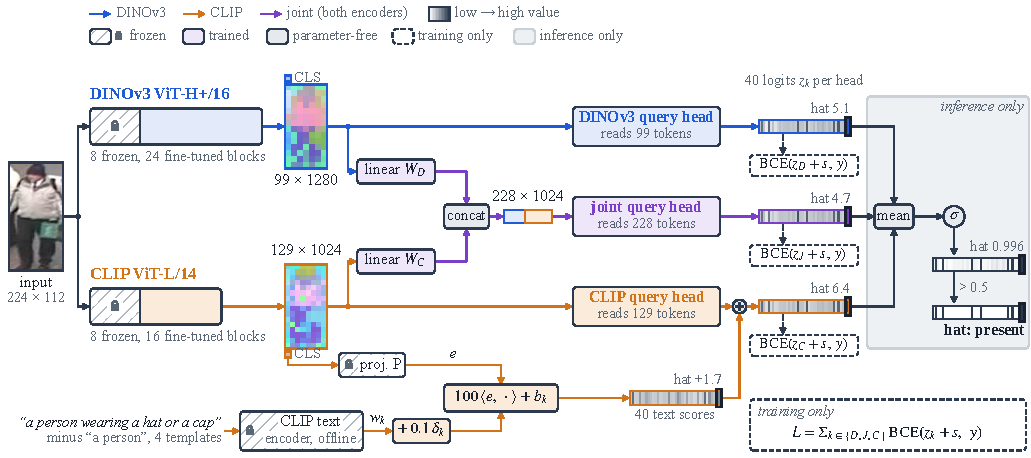
\includegraphics[width=\linewidth]{uniquery_model.pdf}
\caption{UniQuery trên một ảnh PETA. Phần gạch chéo có ổ khoá được đóng băng, màu nhạt là phần được train, ô xám là phép toán không có tham số, và màu các ô token là PCA của patch token. Ở nhánh điểm ngôn ngữ, $P$ là phép chiếu đã pretrain của CLIP, $e$ là CLS token sau phép chiếu và chuẩn hoá, $w_k$ là vector câu của thuộc tính $k$ trừ vector câu \texttt{a person}, còn $\delta_k$ và $b_k$ được học. Lúc train, mỗi query head có loss riêng với độ dịch $s$ (\cref{eq:loss}). Lúc inference, logit của ba query head được lấy trung bình rồi so với ngưỡng 0.5. Mô hình đã nộp đã thấy ảnh này khi train.}
\label{fig:arch}
\end{figure*}

%=====================================================================
\section{Giới thiệu}
\label{sec:intro}

Phân tích người đi bộ có vai trò quan trọng trong giám sát video thông minh và bán lẻ trực tuyến. Một bài toán chính trong đó là nhận dạng thuộc tính người đi bộ (PAR). PAR dự đoán các thuộc tính ngữ nghĩa của từng người từ ảnh, cho ra mô tả dễ hiểu hỗ trợ truy vấn người theo thuộc tính và tái nhận dạng người. Dù đã có nhiều tiến bộ, nhận dạng bền vững vẫn khó vì che khuất, độ phân giải thấp, mất cân bằng nhãn và sự thay đổi về ngoại hình cũng như điều kiện chụp~\cite{rap,upar,labelbalanced}. Bài toán còn khó hơn trên camera chưa từng xuất hiện khi train, vì độ phân giải, góc nhìn và ánh sáng thay đổi, và mỗi dataset train gán nhãn thuộc tính theo quy tắc riêng~\cite{upar}.

Foundation encoder được pretrain trên các tập ảnh lớn và đa dạng~\cite{dinov3,clip} là điểm xuất phát tự nhiên cho sự dịch chuyển này. Chúng thường được dùng cho bài toán downstream bằng cách fine-tune một encoder cùng một head nhỏ, hoặc lấy trung bình logit của nhiều encoder fine-tune riêng rẽ~\cite{deepens}. Các đội UPAR trước đây đi theo những hướng này, với một Swin-B fine-tune riêng~\cite{upar23}, ngưỡng riêng cho từng thuộc tính chọn trên dữ liệu validation~\cite{upar24}, hoặc hai encoder gộp thành một vector dùng chung cho mọi thuộc tính~\cite{c2tnet}. Trung bình của các encoder fine-tune riêng rẽ dùng cùng một tỷ lệ trộn cho mọi thuộc tính, và các encoder của nó không bao giờ được train cùng nhau.

Trong bài báo này, nhóm trình bày cách tiếp cận cho Track~1 của UPAR Challenge 2027. Mô hình của nhóm, UniQuery (\cref{fig:arch}), fine-tune đồng thời DINOv3 và CLIP, và mỗi encoder có một query head riêng. Bên cạnh hai query head này, một joint query head kết hợp đặc trưng của cả hai encoder qua các attribute query riêng cho từng thuộc tính, nhờ đó mỗi thuộc tính lấy được những thông tin khác nhau từ hai encoder. Lúc inference, nhóm lấy trung bình logit của ba query head. Để đánh giá mức độ hiệu quả của phương pháp một cách chặt chẽ, nhóm xây dựng một khung đánh giá, trong đó mọi lựa chọn thiết kế được kiểm tra trên một dataset không có trong dữ liệu train. Các đóng góp chính của bài như sau.
\begin{itemize}
\item Nhóm đề xuất UniQuery, train chung DINOv3 và CLIP và để một query riêng của mỗi thuộc tính quyết định cách trộn hai encoder. UniQuery vượt ensemble của các encoder fine-tune riêng rẽ với cùng loss trên cả hai held-out dataset, và cũng cao hơn trên tập test ẩn dù khoảng chênh ở đó nhỏ. Mức tăng cần joint query head, vì khi bỏ nó lúc inference, trung bình của hai query head còn lại không vượt ensemble.
\item Nhóm cho thấy, trong các thí nghiệm của bài, cách trộn cần được học cùng lúc với việc fine-tune encoder. Các fusion head học trên các encoder đã fine-tune riêng rẽ không vượt trung bình logit đơn giản khi tính trung bình trên hai held-out dataset, và khi đóng băng encoder, UniQuery giảm xuống dưới một DINOv3 fine-tune riêng.
\item Nhóm phân tích cách joint query head trộn hai encoder. Mỗi attention head của nó gần như chỉ đọc token của một encoder, và số attention head dành cho DINOv3 hay CLIP thay đổi theo thuộc tính. Trên phần lớn thuộc tính, joint query head chính xác hơn trung bình của hai query head riêng, và ở các thuộc tính không phải màu, nó thường bằng hoặc vượt query head mạnh hơn.
\end{itemize}

%=====================================================================
\section{Công trình liên quan}
\label{sec:related}

Bài toán xuyên domain và học thống nhất thu hút các nhà nghiên cứu, vì độ chính xác cao trên một dataset PAR riêng lẻ không bảo đảm độ tin cậy ở môi trường mới~\cite{upar,rethinkpar}. Ở mức biểu diễn, ASRL~\cite{asrl} giảm sự nhầm lẫn của bộ phân loại do tương quan giữa các thuộc tính, bằng một đặc trưng riêng cho mỗi thuộc tính và một bộ phân loại trực giao được giữ cố định. AttriVision~\cite{attrivision} fine-tune cả hai encoder của CLIP để embedding ảnh gần với embedding của các câu ngắn mô tả giá trị thuộc tính của ảnh, rồi dự đoán từng thuộc tính bằng độ tương đồng cosine. Giống AttriVision, UniQuery dùng text embedding của CLIP, nhưng giữ text encoder đóng băng và chỉ cộng vào logit của CLIP query head một điểm ngôn ngữ, tính từ độ giống của ảnh với câu mô tả thuộc tính.

Một hướng liên quan dùng ảnh của domain đích. AdaGPAR~\cite{adagpar} giữ nguyên trọng số lúc test và phân loại ảnh mới theo độ tương đồng với các prototype dựng từ những dự đoán đáng tin cậy trên domain đích. LDCD-PAR~\cite{ldcd} train trên cả ảnh đích không nhãn, với một domain discriminator đối kháng trên đặc trưng cục bộ. Ngược lại, UniQuery thuộc hướng domain generalization và không dùng ảnh nào của domain đích.

Học thống nhất là một con đường khác dẫn tới biểu diễn chuyển giao được. UniHCP~\cite{unihcp} train chung một ViT encoder và một decoder cho nhiều bài toán về người, trong đó mỗi bài toán có bộ query riêng và PAR có một query cho mỗi thuộc tính. Phương pháp PATH trong HumanBench~\cite{humanbench} pretrain một encoder dùng chung trên nhiều dataset về người, với một projector riêng cho mỗi bài toán. CLEAR~\cite{clear} dùng lại mạng nhận dạng thuộc tính cho truy vấn người, bằng cách đưa câu mô tả các thuộc tính cần tìm qua một mô hình ngôn ngữ GPT và chỉ train các adapter nhỏ. Như UniHCP và các bộ phân loại đa nhãn dựa trên query~\cite{q2l,mldecoder}, UniQuery dùng các query học được để đọc token của ảnh, nhưng các query trong joint query head đọc token của hai encoder khác nhau.

Hai encoder của UniQuery khác nhau ở cách pretrain. DINOv3~\cite{dinov3} học self-supervised trên ảnh không nhãn và cho patch feature chất lượng cao, còn CLIP~\cite{clip} và các bản kế tiếp~\cite{metaclip,dfn,evaclip,siglip2,pe} học khớp ảnh với chú thích trên dữ liệu web. Độ đa dạng của dữ liệu web là nguồn chính giúp CLIP bền vững khi phân phối dữ liệu thay đổi~\cite{clipdata}. Tuy vậy, CLIP coi một số ảnh khác nhau rõ rệt là giống nhau, trong khi một encoder self-supervised phân biệt được chúng~\cite{eyeswide}. Thêm đặc trưng self-supervised bên cạnh CLIP cải thiện mô hình ngôn ngữ đa phương thức trên các benchmark thiên về thị giác~\cite{eyeswide,cambrian}, nên nhóm ghép DINOv3 với CLIP.

Cách đơn giản để ghép hai encoder là ensemble. Mỗi encoder được fine-tune riêng thành một mô hình, và lúc inference, dự đoán của hai mô hình được lấy trung bình~\cite{deepens}. Ensemble chỉ có lợi ở những ảnh mà hai mô hình dự đoán khác nhau~\cite{krogh}. Nó cũng dùng chung một tỷ lệ trộn cho mọi thuộc tính. Lấy trung bình tham số~\cite{soups,wiseft} không gộp được DINOv3 với CLIP, vì nó cần các mô hình có chung điểm xuất phát. Distillation gộp nhiều encoder vào một~\cite{amradio}, nhưng encoder học trò vẫn thua các teacher của nó ở một số bài toán, ví dụ thua teacher ảnh và văn bản ở zero-shot classification~\cite{amradio,cradio4}. Stacking học cách trộn trên các mô hình đã train xong~\cite{stacking}. Ở UPAR 2024~\cite{upar24}, C$^2$T-Net~\cite{c2tnet} train chung một Swin-B và một EVA ViT-L rồi gộp chúng thành một vector dùng chung cho mọi thuộc tính. UniQuery cũng train chung hai encoder, nhưng mỗi thuộc tính có một query riêng quyết định cách trộn, và mỗi encoder giữ query head riêng.

Các thuộc tính cũng khác nhau về tần suất, và phần lớn trong 40 thuộc tính có ít mẫu dương. Khi train thông thường, mô hình thiên về dự đoán âm cho những thuộc tính này~\cite{logitadj}. Thiên lệch này làm giảm mean balanced accuracy (mA), metric lấy trung bình theo thuộc tính độ chính xác trên mẫu dương và trên mẫu âm với trọng số như nhau. Qua đó nó cũng làm giảm Challenge\_Avg, metric của cuộc thi, là trung bình điều hoà của mA và instance F1. DeepMAR~\cite{deepmar} bù lại bằng cách đánh trọng số loss của mỗi thuộc tính theo tỷ lệ mẫu dương của nó, và UniQuery cũng dùng trọng số này. Các đội UPAR trước đây còn chọn một ngưỡng riêng cho từng thuộc tính trên ảnh validation của domain nguồn~\cite{upar24}, nên các ngưỡng này có thể không đứng vững trên camera mới. Logit adjustment~\cite{logitadj} cộng vào logit một độ dịch theo tần suất của thuộc tính ngay trong loss lúc train, nên UniQuery dùng một ngưỡng 0.5 cho mọi thuộc tính lúc inference.

%=====================================================================
\section{Phương pháp đề xuất}
\label{sec:method}

\begin{figure}[t]
\centering
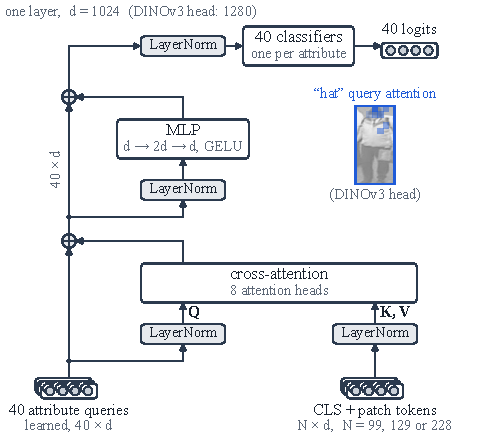
\includegraphics[width=\linewidth]{query_head.pdf}
\caption{Một query head. Ba query head của UniQuery có cùng thiết kế và chỉ khác token mà chúng đọc. Hình nhỏ là attention của query mũ trong DINOv3 query head trên ảnh của \cref{fig:arch}, trung bình tám attention head.}
\label{fig:qhead}
\end{figure}

\Cref{fig:arch} trình bày kiến trúc của UniQuery. Một ảnh người đi bộ đã cắt cỡ $224\times112$ được đưa qua hai encoder là DINOv3 ViT-H+/16~\cite{dinov3} và image encoder OpenAI CLIP ViT-L/14~\cite{clip}, và cả hai được fine-tune trong cùng một mạng. Ba query head đọc token của hai encoder theo ba cách. DINOv3 query head và CLIP query head chỉ đọc token của encoder tương ứng, còn joint query head đọc token của cả hai. Mỗi query head cho ra 40 logit ứng với 40 thuộc tính nhị phân. Lúc train, mỗi query head có loss riêng, còn lúc inference, logit của ba query head được lấy trung bình.

CLIP query head còn dùng khả năng so ảnh với câu chữ mà CLIP học được khi pretrain. Với thuộc tính đội mũ, CLIP so ảnh với câu \texttt{a person wearing a hat or a cap} và với câu \texttt{a person}. Điểm ngôn ngữ của thuộc tính này là độ giống của ảnh với câu thứ nhất trừ đi độ giống với câu thứ hai (\cref{fig:zsidea}). Điểm này được cộng vào logit của thuộc tính đội mũ mà CLIP query head tính từ token của ảnh. Phép trừ nhằm bỏ phần giống chung với câu \texttt{a person} mà câu mô tả nào cũng có, còn phép cộng nhằm đưa hiểu biết của CLIP về thuộc tính vào logit tính từ token của ảnh.

\begin{figure}[t]
\centering
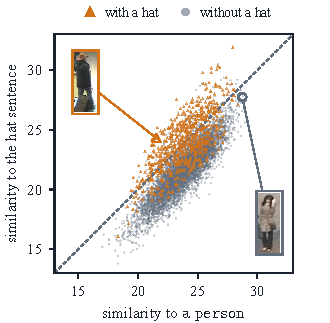
\includegraphics[width=0.68\linewidth]{text_idea.pdf}
\caption{Ý tưởng của điểm ngôn ngữ với thuộc tính đội mũ, trên ảnh validation của PETA. Điểm ngôn ngữ của một ảnh là khoảng cách theo chiều dọc từ điểm của nó tới đường chéo. Ảnh không đội mũ giống câu đội mũ hơn ảnh đội mũ, nhưng nằm dưới đường chéo nên có điểm ngôn ngữ thấp hơn.}
\label{fig:zsidea}
\end{figure}

Token của DINOv3 và của CLIP có độ rộng khác nhau, nên trước khi vào joint query head, mỗi loại token đi qua một lớp linear riêng để về cùng một độ rộng. Sau đó token của hai encoder được nối thành một dãy cho joint query head đọc chung. Bên trong, mỗi query head gồm một lớp cross-attention, một MLP và một bộ phân loại~\cite{q2l,mldecoder} (\cref{fig:qhead}).

Lúc train, loss ở \cref{eq:loss} được áp dụng cho cả ba query head
\begin{equation}
L=\sum_{k\in\{D,J,C\}}\;\sum_{a=1}^{40} m_a\,w_a(y_a)\,\mathrm{BCE}\big(z_{k,a}+s_a,\;y_a\big),
\label{eq:loss}
\end{equation}
trong đó $s_a=\tau\log\frac{p_a}{1-p_a}$, $p_a$ là tần suất của thuộc tính $a$ trong dữ liệu train, và $\tau=0.32$. Độ dịch $s_a$ là logit adjustment~\cite{logitadj} và chỉ được dùng lúc train. Trọng số DeepMAR $w_a(y_a)$~\cite{deepmar} bằng $e^{1-p_a}$ với mẫu dương và $e^{p_a}$ với mẫu âm, nên nó dời ngưỡng quyết định một lượng $1-2p_a$ trên thang logit. Giá trị $\tau=0.32$ được chọn để tổng độ dịch quyết định lúc train, gồm phần $1-2p_a$ do $w_a$ và phần do $s_a$, khớp theo bình phương tối thiểu trên 40 thuộc tính với tổng độ dịch của một quy tắc hậu xử lý. Quy tắc này lấy một mô hình chỉ train với trọng số DeepMAR, rồi cộng $0.42\,\big(\log\frac{1-p_a}{p_a}-(1-2p_a)\big)$ vào logit sau khi train. Hệ số 0.42 của quy tắc này được chọn trên các lần train leave-one-dataset-out. Ký hiệu $D$ là DINOv3 query head, $J$ là joint query head và $C$ là CLIP query head. Ở đây $z_{k,a}$ là logit của query head $k$ cho thuộc tính $a$, và $y_a$ là nhãn sau khi làm mượt với hệ số 0.05. Mask $m_a$ loại bỏ những thuộc tính không được gán nhãn trong dataset chứa ảnh đầu vào.

Lúc train, nhóm đóng băng patch embedding và tám block đầu của mỗi encoder, rồi fine-tune phần còn lại bằng AdamW trong ba epoch, với batch size 64 và trung bình động mũ (EMA) của trọng số. Learning rate là $5\times10^{-5}$ ở block trên cùng, giảm 0.75 lần qua mỗi block bên dưới, và gấp mười lần ở các query head. Mô hình nộp được train trên split train và validation của cả ba dataset. Lúc inference, trung bình logit của ba query head đi qua hàm sigmoid, và thuộc tính được dự đoán là có khi xác suất lớn hơn 0.5. Giống một ensemble của hai encoder train riêng, mỗi ảnh chỉ cần hai lượt chạy encoder, với độ trễ đo được khoảng 3.0\,ms cho mỗi ảnh trên GPU NVIDIA RTX 5090 khi chạy theo batch 128.

%=====================================================================
\section{Thí nghiệm}
\label{sec:exp}

Nhóm đánh giá các mô hình train riêng rẽ, từng query head của UniQuery, và UniQuery với trung bình ba query head. Trung bình ba query head cho Challenge\_Avg trung bình cao hơn từng query head đứng riêng và cao hơn ensemble train riêng, nên nhóm dùng cấu hình này cho bản nộp cuối.

\paragraph{Quy trình đánh giá.} Để mô phỏng các camera chưa từng thấy của tập test ẩn, nhóm đánh giá theo kiểu leave-one-dataset-out. Trong mỗi fold, một dataset được giữ ngoài, và mô hình không thấy ảnh nào của dataset này khi train. Mô hình chỉ được train trên split train của hai dataset còn lại, rồi được chấm trên split validation của dataset bị giữ ngoài. Fold PETA train trên PA100k và Market-1501, rồi được chấm trên 6,963 ảnh validation của PETA. Fold Market train trên PA100k và PETA, rồi được chấm trên 16,458 ảnh validation của Market-1501. Nhóm không dùng fold giữ ngoài PA100k, vì khi bỏ PA100k chỉ còn 18.7 nghìn ảnh train. Metric là Challenge\_Avg, tính theo phần trăm. Mô hình của mỗi fold được train giống mô hình nộp, chỉ khác là dữ liệu train không có split validation. Khi chấm, mỗi ảnh đi qua mô hình một lần, không lật ngang, giống bản nộp, và kết quả là của một seed nếu không ghi khác. Hệ số 0.42 dùng để chọn $\tau$ và encoder đi cùng DINOv3 được chọn trên chính các fold này, nên điểm trên fold có thể hơi lạc quan cho các lựa chọn đó. Tập test ẩn là đánh giá duy nhất không bị các lựa chọn này ảnh hưởng.

\begin{table}[t]
\centering
\small
\setlength{\tabcolsep}{3pt}
\begin{tabular}{@{}lccc@{}}
\toprule
Mô hình & PETA & Market & TB \\
\midrule
DINOv3 train riêng & 81.46 & 86.31 & 83.89 \\
CLIP train riêng & 81.44 & 85.50 & 83.47 \\
Ensemble của hai encoder, seed 1 & 82.45 & 86.30 & 84.38 \\
Ensemble của hai encoder, seed 2 & 82.29 & 86.33 & 84.31 \\
\midrule
UniQuery, chỉ DINOv3 query head & 81.26 & 86.07 & 83.67 \\
UniQuery, chỉ CLIP query head & 81.45 & 85.56 & 83.51 \\
UniQuery, chỉ joint query head & 82.26 & 86.27 & 84.26 \\
UniQuery, DINOv3 và CLIP query head & 82.24 & 86.32 & 84.28 \\
UniQuery, trung bình ba query head & \textbf{82.54} & 86.39 & 84.46 \\
\midrule
Biến thể, seed 1 & 82.53 & \textbf{86.44} & \textbf{84.49} \\
Biến thể, seed 2 & 82.51 & 86.32 & 84.42 \\
Biến thể có hai joint query head & 82.51 & 86.43 & 84.47 \\
\bottomrule
\end{tabular}
\caption{Challenge\_Avg trên held-out dataset, cùng loss ở \cref{eq:loss}. TB là trung bình hai fold, và cấu hình đã nộp là UniQuery với trung bình ba query head. Dòng DINOv3 và CLIP query head lấy trung bình hai query head này của cùng mô hình, không có joint query head. Biến thể cộng thêm điểm ngôn ngữ cho màu quần áo trên vùng thân trên hoặc thân dưới, với một bộ câu mô tả khác, và lúc train ẩn mỗi encoder khỏi joint query head với xác suất 0.25.}
\label{tab:main}
\end{table}

\paragraph{UniQuery so với ensemble train riêng.} \Cref{tab:main} so sánh UniQuery với ensemble của hai encoder train riêng rẽ, dùng cùng kiến trúc encoder và cùng loss. Trung bình logit của ba query head trong UniQuery vượt cả hai seed của ensemble trên cả hai fold. Mức tăng này cần joint query head. Khi bỏ joint query head lúc inference, trung bình của DINOv3 query head và CLIP query head trong UniQuery không còn cao hơn ensemble. Joint query head đứng riêng cao hơn từng single-encoder query head nhưng cũng chưa vượt ensemble. Mức tăng chỉ xuất hiện khi joint query head được lấy trung bình cùng hai single-encoder query head.

\paragraph{Tính nhất quán.} UniQuery chỉ hơn ensemble khoảng 0.08 đến 0.15 điểm trung bình, gần bằng khoảng chênh 0.07 điểm giữa hai seed của ensemble. Vì vậy nhóm kiểm tra xem mức tăng có lặp lại ở các lần train khác hay không. Ba dòng cuối của \cref{tab:main} là ba lần train của một biến thể UniQuery có vài thay đổi nhỏ, ghi trong chú thích của bảng, chứ không phải UniQuery train lại với seed khác. Cả bốn lần train, gồm UniQuery và ba lần của biến thể, đều có điểm trung bình hai fold cao hơn cả hai seed của ensemble. Xét riêng từng fold, bốn lần train này thắng cả 8 so sánh với hai seed của ensemble trên PETA và 7 trong 8 so sánh trên Market.

\begin{figure}[t]
\centering
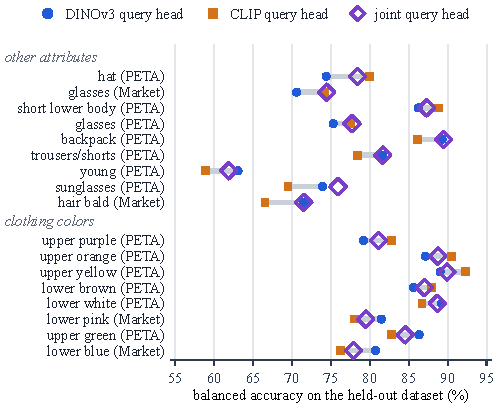
\includegraphics[width=\linewidth]{pick.pdf}
\caption{Joint query head so với hai single-encoder query head, trên các thuộc tính mà hai query head này chênh nhau ít nhất 2 điểm và có ít nhất 50 ảnh dương. Số liệu là trung bình hai seed của biến thể ở \cref{tab:main}.}
\label{fig:pick}
\end{figure}

\begin{figure*}[t]
\centering
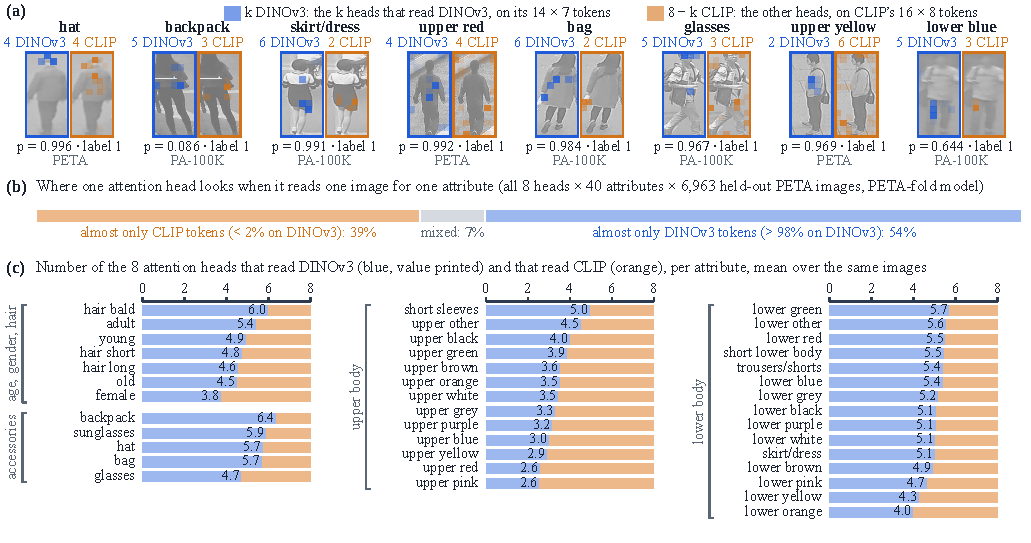
\includegraphics[width=\linewidth]{routing_v2.pdf}
\caption{Cách joint query head dùng hai encoder. (a) Attention của các attention head đọc DINOv3 và đọc CLIP, trên tám ảnh validation mà mô hình đã nộp đã thấy khi train. (b, c) Thống kê trên 6,963 ảnh held-out của PETA, với mô hình fold PETA.}
\label{fig:routing}
\end{figure*}

\paragraph{Trộn riêng cho từng thuộc tính.} Joint query head không trộn hai encoder theo một tỷ lệ chung cho mọi thuộc tính. \Cref{fig:pick} so sánh nó với hai single-encoder query head của biến thể UniQuery ở \cref{tab:main}. Tính trên mọi thuộc tính, hai seed và hai fold, joint query head cao hơn trung bình của hai single-encoder query head ở 82\% trường hợp. Ở các thuộc tính không phải màu, như tuổi, giới tính, tóc, kiểu quần áo và phụ kiện, nó bằng hoặc vượt query head tốt hơn ở 69\% trường hợp, ví dụ với ba lô, kính râm hay quần dài và quần ngắn. Ở màu quần áo, tỷ lệ này chỉ là 40\%, và joint query head thường nằm giữa hai query head. Attention của joint query head cho thấy nó chia việc giữa hai encoder theo thuộc tính (\cref{fig:routing}). Trên ảnh held-out của PETA, ở 93\% số lần một attention head đọc một ảnh cho một thuộc tính, hơn 98\% attention của nó rơi vào token của cùng một encoder (\cref{fig:routing}b). Vì vậy với mỗi thuộc tính, có thể đếm số attention head trong tám attention head đọc DINOv3. Một attention head được coi là đọc DINOv3 khi hơn nửa attention của nó rơi vào token DINOv3 (\cref{fig:routing}c). Ba lô dùng trung bình 6.4 trong tám attention head cho DINOv3, còn áo đỏ và áo hồng chỉ dùng khoảng 2.6. Nhìn chung, thuộc tính thân dưới và phụ kiện dựa nhiều hơn vào DINOv3, còn màu áo dựa nhiều hơn vào CLIP.

\paragraph{Vì sao chọn DINOv3 và CLIP?} \Cref{tab:two} cho thấy encoder thứ hai nên khác encoder thứ nhất. Bản fine-tune thứ hai của cùng một encoder thêm tối đa 0.10 điểm trung bình, còn một encoder khác thêm 0.4 đến 0.6 điểm. Mức tăng này đến từ PETA. Trên Market, ghép thêm CLIP giúp ít hơn nhiều, và với $\tau=0.42$ cặp DINOv3 và CLIP còn thấp hơn DINOv3 đứng riêng. Giả thuyết của nhóm là hai encoder pretrain theo hai cách khác nhau ít cùng dự đoán sai trên một ảnh hơn hai bản fine-tune của cùng một encoder. Để kiểm tra, nhóm lấy các cặp ảnh và thuộc tính mà một mô hình dự đoán sai, đo tỷ lệ mô hình kia cũng sai trên các cặp đó, rồi lấy trung bình theo hai chiều. Hai bản fine-tune của cùng một encoder trong \cref{tab:two} trùng 89\% đến 93\% số lỗi, còn DINOv3 và CLIP chỉ trùng 72\% trên PETA và 77\% trên Market-1501. Để chọn encoder đi cùng DINOv3, nhóm thử 12 encoder trên fold PETA, gồm CLIP, AIMv2~\cite{aimv2}, EVA02-CLIP~\cite{evaclip}, MetaCLIP2~\cite{metaclip2}, MobileCLIP2~\cite{mobileclip2}, DFN-CLIP~\cite{dfn}, hai bản PE~\cite{pe} và bốn bản SigLIP2~\cite{siglip2}. Mỗi encoder được fine-tune riêng rồi lấy trung bình logit với DINOv3. Encoder nào cũng chỉ trùng 66\% đến 72\% số lỗi với DINOv3, nên điểm của cặp đi theo điểm của encoder thứ hai khi đứng riêng. Khi đứng riêng, CLIP hơn mọi encoder còn lại ít nhất 0.5 điểm, và qua năm lần train CLIP, cặp DINOv3 và CLIP đạt từ 81.04\% đến 81.23\%. Chỉ cặp với AIMv2-L rơi vào khoảng này, còn 10 encoder kia đều cho cặp thấp hơn. Công thức train được chỉnh trên DINOv3 và CLIP, nên có thể chưa hợp với các encoder khác. Trong chính UniQuery, thay CLIP bằng SigLIP2-L/16 hoặc C-RADIOv4-H~\cite{cradio4}, hay thay DINOv3 bằng C-RADIOv4-H, đều làm Challenge\_Avg trung bình hai fold giảm (\cref{tab:swap}). Mức giảm chủ yếu nằm ở PETA. Trên Market, cặp với SigLIP2-L cũng thấp hơn, còn hai cặp có C-RADIOv4-H nhỉnh hơn UniQuery.

\begin{table}[t]
\centering
\small
\setlength{\tabcolsep}{4pt}
\begin{tabular}{@{}lccc@{}}
\toprule
Encoder (trung bình logit) & PETA & Market & TB \\
\midrule
\multicolumn{4}{@{}l}{\emph{Loss logit-adjusted, $\tau=0.42$}} \\
CLIP & 81.79 & 85.72 & 83.75 \\
CLIP + CLIP (hai seed) & 81.80 & 85.78 & 83.79 \\
DINOv3 & 81.14 & \textbf{86.78} & 83.96 \\
DINOv3 + CLIP & \textbf{82.29} & 86.49 & \textbf{84.39} \\
\midrule
\multicolumn{4}{@{}l}{\emph{Weighted BCE}} \\
CLIP & 80.68 & 85.01 & 82.84 \\
CLIP + CLIP (hai seed) & 80.69 & 85.12 & 82.90 \\
DINOv3 & 80.49 & 85.31 & 82.90 \\
DINOv3 + DINOv3 (hai lần train) & 80.66 & 85.35 & 83.00 \\
DINOv3 + CLIP & \textbf{81.08} & \textbf{85.54} & \textbf{83.31} \\
\bottomrule
\end{tabular}
\caption{Challenge\_Avg trên held-out dataset của các encoder fine-tune riêng rồi lấy trung bình logit. Các lần train này thuộc giai đoạn trước, với $\tau=0.42$ thay cho 0.32 trong \cref{eq:loss}, hoặc với weighted BCE (\cref{eq:loss} không có $s_a$), vì chỉ giai đoạn này có hai bản fine-tune của cùng một encoder. Hai bản DINOv3 là hai lần train cùng công thức.}
\label{tab:two}
\end{table}

\begin{table}[t]
\centering
\small
\setlength{\tabcolsep}{2pt}
\begin{tabular}{@{}lcccc@{}}
\toprule
Cách trộn hai mô hình & PETA & Market & TB & Nguồn \\
\midrule
Trung bình logit, không học thêm & \textbf{82.45} & 86.30 & \textbf{84.38} & 89.46 \\
Học tỷ lệ trộn mỗi thuộc tính & 82.43 & \textbf{86.31} & 84.37 & 89.49 \\
\midrule
\multicolumn{5}{@{}l}{\emph{Trung bình logit cộng hiệu chỉnh học từ}} \\
\quad attribute vector của DINOv3 & 81.15 & 85.99 & 83.57 & 90.93 \\
\quad attribute vector của CLIP & 81.55 & 86.06 & 83.81 & 90.52 \\
\quad cả hai, nối lại qua một MLP & 81.27 & 85.92 & 83.60 & 91.02 \\
\quad cả hai, tỷ lệ riêng mỗi thuộc tính & 81.25 & 85.95 & 83.60 & 90.97 \\
\quad cả hai, tỷ lệ theo từng ảnh & 81.01 & 85.86 & 83.44 & 91.14 \\
\bottomrule
\end{tabular}
\caption{Học cách trộn trên hai mô hình đã fine-tune riêng của ensemble, được giữ cố định (Challenge\_Avg trên held-out dataset). Phần hiệu chỉnh tính bằng một lớp linear, bắt đầu bằng 0, và được train với loss ở \cref{eq:loss} trên 85\% ảnh validation của hai dataset nguồn (khoảng 22 nghìn ảnh ở fold PETA và 14 nghìn ảnh ở fold Market). Cột Nguồn là Challenge\_Avg trung bình hai fold trên 15\% ảnh nguồn còn lại, mà fusion head không thấy khi train.}
\label{tab:frozen}
\end{table}

\paragraph{Có học được cách trộn sau khi train không?} Ensemble train riêng trộn hai mô hình bằng cách lấy trung bình logit, với cùng tỷ lệ một nửa cho mọi thuộc tính. Nhóm kiểm tra xem có thể học một cách trộn tốt hơn sau khi hai mô hình đã train xong hay không, mà không cần train chung như UniQuery. Hai mô hình được giữ nguyên, và chỉ một fusion head nhỏ đặt trên đầu ra của chúng được train (\cref{tab:frozen}). Loại fusion head thứ nhất chỉ học cho mỗi thuộc tính một tỷ lệ trộn hai logit. Năm loại còn lại cộng thêm vào trung bình logit một phần hiệu chỉnh, tính từ attribute vector của query head. Attribute vector là vector mà query head tạo ra cho mỗi thuộc tính ngay trước bộ phân loại. Tính theo điểm trung bình hai fold, không fusion head nào vượt trung bình logit thông thường, và năm loại có phần hiệu chỉnh còn làm Challenge\_Avg giảm 0.6 đến 0.9 điểm. Các fusion head không thua vì học kém. Trên ảnh nguồn mà chúng không thấy khi train, năm loại này vượt trung bình logit từ 1.1 đến 1.7 điểm. Như vậy với các fusion head nhóm đã thử, cách trộn học sau khi train chỉ đúng với dataset nguồn và không chuyển sang được dataset mới. Đây là lý do UniQuery học cách trộn ngay trong lúc train hai encoder.

\begin{table}[t]
\centering
\small
\setlength{\tabcolsep}{3pt}
\begin{tabular}{@{}llccc@{}}
\toprule
Cặp encoder & Cách train & PETA & Market & TB \\
\midrule
DINOv3 + CLIP (đã nộp) & fine-tune & \textbf{82.54} & 86.39 & \textbf{84.46} \\
DINOv3 + CLIP & đóng băng & 81.07 & 85.80 & 83.43 \\
\midrule
C-RADIOv4-H + CLIP & fine-tune & 81.87 & 86.43 & 84.15 \\
DINOv3 + C-RADIOv4-H & fine-tune & 82.11 & \textbf{86.50} & 84.31 \\
DINOv3 + SigLIP2-L & fine-tune & 81.81 & 86.07 & 83.94 \\
\bottomrule
\end{tabular}
\caption{Đóng băng hoặc thay encoder của UniQuery (Challenge\_Avg trên held-out dataset). Khi đóng băng, chỉ 32.6 triệu tham số được train.}
\label{tab:swap}
\end{table}

\paragraph{Encoder có bắt buộc phải fine-tune không?} BRAVE~\cite{brave} giữ nguyên trọng số pretrain của nhiều encoder và chỉ train một module có các query học được để đọc token của chúng. Nhóm thử cách này với UniQuery, bằng cách đóng băng cả hai encoder và chỉ train ba query head cùng hai lớp linear. Khi đó UniQuery mất 1.0 điểm trung bình và thấp hơn cả DINOv3 fine-tune riêng (\cref{tab:swap}). CLIP query head mất 2.7 điểm, còn DINOv3 query head chỉ mất 0.6 điểm. Vì vậy trong bài toán này, encoder cần được fine-tune, và CLIP chịu ảnh hưởng nhiều hơn DINOv3 khi bị đóng băng.

\begin{figure}[t]
\centering
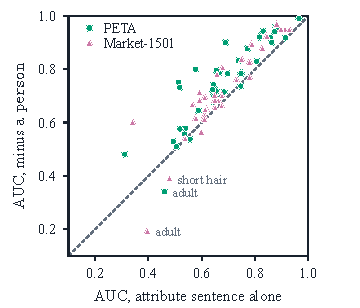
\includegraphics[width=0.74\linewidth]{text_auc.pdf}
\caption{AUC zero-shot của điểm ngôn ngữ trên ảnh validation, mỗi điểm một thuộc tính. Các điểm thấp hơn đường chéo quá 0.05 được ghi tên.}
\label{fig:zsauc}
\end{figure}

\paragraph{Điểm ngôn ngữ của CLIP có giúp không?} Câu mô tả thuộc tính nào cũng nói về một người, nên độ giống của ảnh với câu thuộc tính chứa một phần chung với độ giống của ảnh với câu \texttt{a person}. Phần chung này chỉ đo mức độ ảnh giống một người, không cho biết người đó có thuộc tính hay không. Trừ nó đi sẽ giữ lại phần riêng của thuộc tính. \Cref{fig:zsauc} kiểm tra điều này trước khi train bằng AUC (area under the ROC curve). AUC là xác suất một ảnh có thuộc tính nhận điểm cao hơn một ảnh không có thuộc tính. Trên PETA, phép trừ nâng AUC trung bình từ 0.68 lên 0.76 và làm AUC tăng ở 37 trong 40 thuộc tính, và Market-1501 cho kết quả cùng chiều. Sau khi train, lợi ích nhỏ hơn nhiều. Bỏ điểm ngôn ngữ chỉ làm Challenge\_Avg giảm 0.15 điểm ở PETA và 0.05 điểm ở Market, cùng cỡ với khoảng chênh giữa hai seed. Một cách giải thích là khi CLIP được fine-tune trên dữ liệu có nhãn, CLIP query head học được phần lớn thông tin này trực tiếp từ token của ảnh. Vì vậy điểm ngôn ngữ mang thông tin đúng về thuộc tính nhưng chỉ là một thành phần phụ, không phải nguồn chính của mức tăng của UniQuery.

\begin{table}[t]
\centering
\small
\setlength{\tabcolsep}{3pt}
\begin{tabular}{@{}llc@{}}
\toprule
Bản nộp & Loss & Challenge\_Avg \\
\midrule
Ensemble train riêng & weighted BCE$^\dagger$ & 0.7893 \\
Ensemble train riêng & logit-adjusted & 0.7989 \\
UniQuery, biến thể & logit-adjusted & 0.7992 \\
UniQuery (bản nộp) & logit-adjusted & 0.8001 \\
\bottomrule
\end{tabular}
\caption{Tập test ẩn của UPAR 2027 Track 1, thang 0 đến 1. Mô hình cuối được train trên split train và validation của cả ba dataset. Mọi bản nộp dùng ngưỡng 0.5, không có bước hậu xử lý, và biến thể là biến thể ở \cref{tab:main}. $^\dagger$Có WiSE-FT~\cite{wiseft} cho CLIP.}
\label{tab:test}
\end{table}

\paragraph{Tập test ẩn.} Trên tập test ẩn, cả hai bản UniQuery đều cao hơn ensemble train riêng dùng cùng loss (\cref{tab:test}). Các khoảng chênh này chỉ cỡ khoảng chênh giữa hai bản UniQuery, nên tập test ẩn cho cùng chiều với held-out dataset nhưng không đủ để đo độ lớn của mức tăng. Bản nộp cuối của nhóm là UniQuery.

%=====================================================================
\section{Hạn chế}
\label{sec:limits}

Các kết quả của bài được đo trong bài toán PAR của UPAR 2027, với ba dataset PA100k, PETA, Market-1501 và bộ 40 thuộc tính của cuộc thi. Nhóm chưa kiểm tra UniQuery trên các dataset PAR khác, trên các bài toán khác về người, hay với những cặp encoder khác ngoài các cặp có trong bài. Vì vậy chưa thể khẳng định cách trộn theo từng thuộc tính mang lại lợi ích tương tự trong những bối cảnh đó. Ngoài ra, phần lớn kết quả chỉ có một seed.

%=====================================================================
\section{Kết luận}
\label{sec:conclusion}

Bài báo này nghiên cứu cách kết hợp hai foundation encoder cho nhận dạng thuộc tính người đi bộ trên camera chưa từng thấy. DINOv3 và CLIP ít cùng dự đoán sai trên một ảnh hơn hai bản của cùng một encoder, phù hợp với việc chúng được pretrain theo hai cách khác nhau, và ghép chúng có lợi hơn ghép hai bản như vậy. UniQuery fine-tune hai encoder trong cùng một mạng và để một query riêng cho mỗi thuộc tính quyết định lấy thông tin từ encoder nào. Phát hiện chính của bài là cách trộn cần được học cùng lúc với encoder, qua một joint query head đặt cạnh query head riêng của mỗi encoder. Bỏ joint query head lúc inference thì UniQuery không còn vượt ensemble, còn các cách trộn nhóm thử trên những mô hình đã train xong chỉ khớp với dataset nguồn. Bên trong joint query head, mỗi attention head chọn hẳn một encoder, với thuộc tính thân dưới và phụ kiện nghiêng về DINOv3, còn màu áo nghiêng về CLIP. Với PAR xuyên domain, kết quả này gợi ý nên để mô hình tự phân công encoder cho từng thuộc tính ngay trong lúc train, thay vì trộn các mô hình đã train xong theo một tỷ lệ chung.

{\small
\bibliographystyle{ieeenat_fullname}
\bibliography{refs}
}

\end{document}
